This project aims to implement a Simultaneous Localization and Mapping (SLAM) algorithm on a TurtleBot3 Waffle Pi robot using the Robot Operating System 2 (ROS2) framework for the purpose of autonomous environment mapping, localization, and navigation. SLAM is important for autonomous vehicles as it allows a vehicle to map a room and localize itself in it at the same time. The use of ROS2 allows the robot to be programmed using a combination of both Python and C++.

As shown in Figure \ref{fig:turtlebot3}, the TurtleBot3 is equipped with many components including a Raspberry Pi 4 (small computer) for onboard processing, a differential drive system, and a 360° 2D LiDAR sensor for observations. Due to the limitations of the onboard computer, the robot (client) relies on an external computer (server) for most processing tasks. The server processes data obtained by the robot's LiDAR sensor and transmits control parameters back to it at very fast regular intervals. These control parameters are the linear and angular velocities ($v,\omega$) of the robot that control the differential drive system. This driving system consists of two wheels, one on each side, that can be controlled independently, allowing the robot to turn by having one wheel turn more slowly than the other \parencite{corkeRoboticsVisionControl2023}. The LiDAR sensor, which constantly rotates to observe around the robot, measures distances by "[emitting] short pulses of infrared laser light and [measuring] the time for the reflected pulses to return" \parencite{corkeRoboticsVisionControl2023}.

\begin{figure}[htb]
    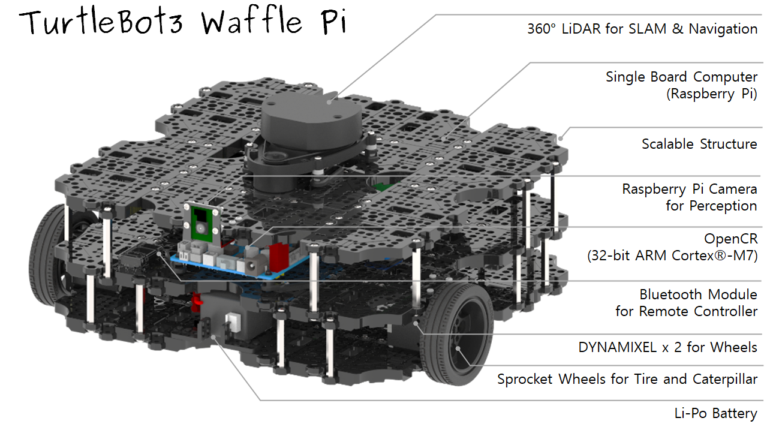
\includegraphics[width=8cm]{turtlebot3.png}
    \centering
    \caption{Components of the TurtleBot3 Waffle Pi \parencite{ROBOTISEManual}.}
    \label{fig:turtlebot3}
\end{figure}

Many optimization algorithms are used in this project. These algorithms often need to use the gradient to iteratively optimize functions. For a multivariable function, the gradient at a given point is a vector with a direction pointing in the direction of fastest increase and a magnitude representing the slope in that direction \parencite{Gradient2024}.
For a point $p = (x_1,\hdots, x_n)$ in $\mathbb{R}^n$, the gradient is given by
\[
    \nabla f(p)=\begin{bmatrix}
        \frac{\partial f}{\partial x_1}(p) \\[6pt]
        \vdots                             \\[6pt]
        \frac{\partial f}{\partial x_n}(p)
    \end{bmatrix}.
\]

In this paper, many robotics related terms are used. The pose refers to an object's position and orientation. Odometry is the travel distance and direction measurements done by wheel encoders \parencite{corkeRoboticsVisionControl2023}. Deadreckoning is the process of estimating the pose from the odometry. \todo{Maybe annex?}